\title{Tendon Robot Statics Model Variants}
\author{John Till}
\date{}

\documentclass[12pt]{article}

\usepackage[a4paper, margin=0.75in]{geometry}
\usepackage[colorlinks=true,urlcolor=blue]{hyperref}
\usepackage{amsmath,amssymb}
\usepackage{graphicx}

\usepackage{xcolor}
\definecolor{OffWhite}{rgb}{0.93,0.93,0.93}
\definecolor{QtCommentColor}{rgb}{0,0.5,0}
\definecolor{QtKeywordColor}{rgb}{0.5,0.5,0}
\definecolor{QtPurpleColor}{rgb}{0.5,0,0.5}
\definecolor{QtGlobal}{rgb}{0.808,0.361,0}
\definecolor{QtFunctionColor}{rgb}{0,0.404,0.486}

\usepackage[T1]{fontenc} %for upquotes in listings
\usepackage{textcomp} %for upquotes in listings
\usepackage{listings}
\lstset{
		language=C++,
		escapeinside={!-}{-!},
		upquote=true,
		%
		otherkeywords={Vector3d, DiagonalMatrix, VectorXd, Matrix3d, Map, MatrixXd, Vector6d, Vector4d,
		              Matrix6d, Eigen, Upper, std, fstream, Matrix3Xd,
									UnitX, pow, inverse, transposeMultiply, segment, data, UnitZ, cross, hat_squared,
									hat_postmultiply, hat_premultiply, normalized,
									Zero, Identity, UnitY, cosseratRodOde, ode4, cols, row, main, shootingFunction,
									block, rotation_error, solveLevenbergMarquardt, cos, sin, toDenseMatrix,
									selfadjointView, llt, close, kirchhoffTendonRobotOde, cwiseProduct, cwiseMin,
									cwiseMax, getRouting},
    morekeywords=[2]{Vector3d, DiagonalMatrix, VectorXd, Matrix3d, Map, MatrixXd, Vector6d, Vector4d,
		                 Matrix6d, Eigen, Upper, std, fstream, Matrix3Xd},
		morekeywords=[3]{UnitX, UnitZ, pow, inverse, transposeMultiply, segment, data, cross, hat_squared,
		                 hat_postmultiply, hat_premultiply, normalized,
		                 Zero, Identity, UnitY, cosseratRodOde, ode4, cols, row, main, shootingFunction,
										 block, rotation_error, solveLevenbergMarquardt, cos, sin, toDenseMatrix,
										 selfadjointView, llt, close, kirchhoffTendonRobotOde, cwiseProduct, cwiseMin,
										 cwiseMax, getRouting},
    %
		frame = single,
		rulecolor=\color{black},
    tabsize=4, % tab space width
    showstringspaces=false, % don't mark spaces in strings
		%
		basicstyle=\footnotesize,%\color{QtIdentifier},
		backgroundcolor=\color{OffWhite},
    commentstyle=\color{QtCommentColor}, % comment color
    keywordstyle=\color{QtKeywordColor}, % keyword color
		keywordstyle=[2]{\color{QtPurpleColor}},
		keywordstyle=[3]{\color{QtFunctionColor}},
    stringstyle=\color{QtCommentColor} % string color
}

\begin{document}

\makeatletter
\renewcommand{\@maketitle}{
\newpage
\null
\vskip 2em
\begin{center}
{\LARGE \@title \par}
\end{center}
\par
} \makeatother

\maketitle

In the last example we implemented a relatively simple tendon robot model where the backbone was modeled as a Cosserat rod and the tendons were routed in parallel with the backbone. There is a plethora of potential modifications to the model, and three potential variations are considered in different sections here.

\section{Kirchhoff Rod Backbone}

There are significant simplifications to the model if we neglect the shear and extension modes as described in \href{https://ieeexplore.ieee.org/document/5957337}{``Statics and Dynamics of Continuum Robots With General Tendon Routing and External Loading''}. This results in $\boldsymbol{v} = \boldsymbol{e}_3$, which is the elastic rod problem as studied by Gustav Kirchhoff prior to the Cosserat brothers. The result for the tendon robot is that one only needs to solve a 3x3 linear system for $\dot{\boldsymbol{u}}$ instead of the 6x6 linear system considered previously for $\dot{\boldsymbol{v}}$ and $\dot{\boldsymbol{u}}$.

The state vector has $\boldsymbol{n}^b$ instead of $\boldsymbol{v}$, and the ODE function is changed accordingly:
\begin{lstlisting}
void kirchhoffTendonRobotOde(VectorXd& y_s_out, VectorXd& y){
    //Unpack state vector
    Matrix3d R = Map<Matrix3d>(&y[3]);
    Vector3d nb = Map<Vector3d>(&y[12]);
    Vector3d u = Map<Vector3d>(&y[15]);
\end{lstlisting}
Of course calculations involving shear or extension are modified so that $\boldsymbol{v} = \boldsymbol{e}_3$. The ODEs are also changed so that there is only a 3x3 linear system as in Equation (17):
\begin{lstlisting}
    //Pack state vector derivative
    Map<Vector3d> p_s(&y_s_out[0]);
    Map<Matrix3d> R_s(&y_s_out[3]);
    Map<Vector3d> nb_s(&y_s_out[12]);
    Map<Vector3d> u_s(&y_s_out[15]);

    //ODEs
    p_s = R.col(2);
    R_s = hat_postmultiply(R,u);
    u_s = H.inverse()*(-u.cross(Kbt*u) - Vector3d::UnitZ().cross(nb) - b);
    nb_s = -u.cross(nb) - G*u_s - a - transposeMultiply(R,rho*area*g);
}
\end{lstlisting}
An inverse is used instead of a linear solver because Eigen has specialized methods to take efficient inverses of small fixed-size matrices.
We also make some minor changes to the objective function since $\boldsymbol{n}^b$ is a state variable instead of $\boldsymbol{v}$:
\begin{lstlisting}
y0 << p0, Map<VectorXd>(Matrix3d(R0).data(), 9), guess;

//Numerically integrate the Cosserat rod equations
Y = ode4<kirchhoffTendonRobotOde>(y0, L);

//Find the internal forces in the backbone prior to the final plate
Vector3d nb = Y.block<3,1>(12,Y.cols()-1);
Vector3d uL = Y.block<3,1>(15,Y.cols()-1);
Vector3d mb = Kbt*uL;
\end{lstlisting}
If we rendered the solution, we would see no visible difference compared the Cosserat model.

\section{Non-parallel Tendon Routing}

The examples so far have assumed the tendons are routed parallel with the backbone. However, the model in
\href{https://ieeexplore.ieee.org/document/5957337}{``Statics and Dynamics of Continuum Robots With General Tendon Routing and External Loading''} is formulated for any general routing path, and helical routing strategies are demonstrated. The Cosserat backbone model is altered to have a helical routing strategy here.

There are a multitude of options for how to represent the tendon routing functions. Lambda functions might be the most straightforward way, and if we were willing to implement our own numerical integration function, the most efficient way would be to precompute all the values at grid points. The approach here is somewhere in between; we'll calculate all the vectors at a given point on the backbone:
\begin{lstlisting}
//Helical routing
const double offset = 0.01506;
void getRouting(double arclength, Vector3d* r, Vector3d* r_s, Vector3d* r_ss){
    const double f = 2*pi/L; //tendons make a full revolution

    double c = offset*cos(f*arclength);
    double s = offset*sin(f*arclength);
    double fc = f*c;
    double fs = f*s;
    double ffc = f*fc;
    double ffs = f*fs;

    r[0] = Vector3d(c, s, 0);
    r[1] = Vector3d(-s, c, 0);
    r[2] = Vector3d(-c, -s, 0);
    r[3] = Vector3d(s, -c, 0);

    r_s[0] = Vector3d(-fs, fc, 0);
    r_s[1] = Vector3d(-fc, -fs, 0);
    r_s[2] = Vector3d(fs, -fc, 0);
    r_s[3] = Vector3d(fc, fs, 0);

    r_ss[0] = Vector3d(-ffc, -ffs, 0);
    r_ss[1] = Vector3d(ffs, -ffc, 0);
    r_ss[2] = Vector3d(ffc, ffs, 0);
    r_ss[3] = Vector3d(-ffs, ffc, 0);
}
\end{lstlisting}
The tendons are still separated by $90^\circ$, but they are routed in helices around the backbone with a frequency ``f''. There are three arrays passed in having four vectors each. ``r'', ``r\_s'', and ``r\_ss'' are set based on the arc length. The ODE includes the derivatives of $\boldsymbol{r}$:
\begin{lstlisting}
Vector3d r[num_tendons], r_s[num_tendons], r_ss[num_tendons];
getRouting(s, r, r_s, r_ss);

for(int i = 0; i < num_tendons; i++){
    Vector3d ri = r[i];
    Vector3d ri_s = r_s[i];
    Vector3d ri_ss = r_ss[i];

    Vector3d pb_si = u.cross(ri) + ri_s + v;
    double pb_s_norm = pb_si.!-\textcolor{QtFunctionColor}{norm}-!();
    Matrix3d A_i = -hat_squared(pb_si)*(tau(i)/pow(pb_s_norm,3));
    Matrix3d G_i = -hat_postmultiply(A_i,ri);
    Vector3d a_i = A_i*(u.cross(pb_si + ri_s) + ri_ss);
\end{lstlisting}
The tendon routing vectors are calculated for the current arclength ``s'' before setting up the linear system. Over in the objective function, we also need to use the tendon routing vectors at the tip when finding the equilibrium error:
\begin{lstlisting}
//Find the equilibrium error at the tip, considering tendon forces
Vector3d force_error = -nb;
Vector3d moment_error = -mb;
Vector3d r[num_tendons], r_s[num_tendons], r_ss[num_tendons];
getRouting(L, r, r_s, r_ss);
for(int i = 0; i < num_tendons; i++){
    Vector3d pb_si = uL.cross(r[i]) + r_s[i] + vL;
    Vector3d Fb_i = -tau(i)*pb_si.normalized();
    force_error += Fb_i;
    moment_error += r[i].cross(Fb_i);
}
\end{lstlisting}
Then we can solve the problem and visualize the effects of helical routing:
\begin{figure}[h]
	\centering
		\includegraphics[width=0.8\textwidth]{fig/Helical.jpg}
\end{figure}

We could also implement a converging tendon strategy like in the paper \href{https://ieeexplore.ieee.org/document/8606257}{``Continuum Robot Stiffness Under External Loads and Prescribed Tendon Displacements''}. We revise the tendon function:
\begin{lstlisting}
//Converging routing
const double offset = 0.01506;
const double routing_slope = -offset/L;
void getRouting(double s, Vector3d* r, Vector3d* r_s, Vector3d* r_ss){
    double b = (1 - s/L)*offset;

    r[0] = Vector3d(b, 0, 0);
    r[1] = Vector3d(0, b, 0);
    r[2] = Vector3d(-b, 0, 0);
    r[3] = Vector3d(0, -b, 0);

    r_s[0] = Vector3d(routing_slope, 0, 0);
    r_s[1] = Vector3d(0, routing_slope, 0);
    r_s[2] = Vector3d(-routing_slope, 0, 0);
    r_s[3] = Vector3d(0, -routing_slope, 0);

    r_ss[0] = r_ss[1] = r_ss[2] = r_ss[3] = Vector3d(0, 0, 0);
}
\end{lstlisting}
Then solving with converging routing yields the following solution:
\begin{figure}[h]
	\centering
		\includegraphics[width=0.8\textwidth]{fig/Converging.jpg}
\end{figure}

\section{Tendon Displacement Control}

In the examples so far, the forward kinematics input has been the tendon tensions. However, most actuator control position instead of force. This scenario is also considered in the paper \href{https://ieeexplore.ieee.org/document/8606257}{``Continuum Robot Stiffness Under External Loads and Prescribed Tendon Displacements''}. There are additional unknowns since the tendon tensions are not given, and additional constraints since the backbone must take a shape so that the tendon lengths are correct. For example, increasing the distance $q_i$ the tendon extends below the baseplate will cause the backbone to bend so that the arc length of the tendon above the baseplate is reduced, and the total tendon length remains constant (assuming an inextensible tendon).

\begin{figure}[h]
	\centering
		\includegraphics[width=0.5\textwidth]{fig/DisplacementControl.jpg}
\end{figure}

We declare additional independent parameters for the displacement control:
\begin{lstlisting}
const VectorXd q = Vector4d(5e-3, 0, -5e-3, 0);
const VectorXd l_star = Vector4d(L,L,L,L);
\end{lstlisting}
The length a tendon extends behind the baseplate is $q_i$, and the total length of a tendon before stretching is $l_i^*$. We're careful when setting the actuator displacements because it is especially easy to have an \emph{ill-posed} problem. For instance, pulling all the tendons back by half the length of the backbone is simply not realistic, and the solver would probably fail to find a solution.
The tendon tensions are now dependent variables, so they are declared as static:
\begin{lstlisting}
static VectorXd tau;
\end{lstlisting}
These tensions will be guessed, so we change the guess initialization in the main function:
\begin{lstlisting}
VectorXd init_guess = VectorXd::Zero(6 + num_tendons); //nb, u, and tau
\end{lstlisting}
and we unpack the last elements of the guess as the tendon tensions:
\begin{lstlisting}
tau = guess.segment<num_tendons>(6);
\end{lstlisting}
Based on how the backbone deforms, each tendon will have some arc length it is routed along the backbone, with errors resulting from incorrect lengths. Calculating the errors requires modifying the ODE function to also integrate the tendon arc lengths. We extend the state vector so that the last entries are the tendon arc lengths: 
\begin{lstlisting}
Map<VectorXd> pb_s_norm(&y_s_out[18], num_tendons);
\end{lstlisting}
Now the change in tendon arc length with respect to the change in reference arc length is stored as part of the state vector derivative:
\begin{lstlisting}
pb_s_norm(i) = pb_si.!-\textcolor{QtFunctionColor}{norm}-!();
Matrix3d A_i = -hat_squared(pb_si)*(tau(i)/pow(pb_s_norm(i),3));
\end{lstlisting}
We modify the initial conditions to include the arc lengths of the tendons behind the base plate:
\begin{lstlisting}
VectorXd y0(18+num_tendons);
y0 << p0, Map<VectorXd>(Matrix3d(R0).data(),9), v0, u0, q;
\end{lstlisting}
Then we have some error in the integrated lengths of the tendons versus the known lengths specified as design parameters:
\begin{lstlisting}
//Find the length violation error
VectorXd integrated_lengths = Y.block<num_tendons,1>(18,Y.cols()-1);
VectorXd length_error = integrated_lengths - l_star;

VectorXd distal_error(6 + num_tendons);
distal_error << force_error, moment_error, length_error;
\end{lstlisting}

Now if we run the program, the robot is solved using tendon displacement as the forward kinematics input. However, our approach currently assumes the tendons are inextensible and capable of supporting compression. We address the former first by adding compliance as an independent variable:
\begin{lstlisting}
const VectorXd C = Vector4d(1e-4,1e-4,1e-4,1e-4);
\end{lstlisting}
Then the length error is revised to include the tendon stretch, which is calculated from Hooke's law:
\begin{lstlisting}
VectorXd stretch = l_star.cwiseProduct( C.cwiseProduct(tau) );
VectorXd length_error = integrated_lengths - (l_star + stretch);
\end{lstlisting}
Now the tendons will stretch under tension. Unfortunately, they will also contract under compression. 
To disallow compression, we include the effects of slack. Since slack and tension are mutually exclusive effects, we use a single variable to represent them both when we unpack the guess:
\begin{lstlisting}
tau = guess.segment<num_tendons>(6).cwiseMax(0);
VectorXd slack = -(guess.segment<num_tendons>(6).cwiseMin(0));
\end{lstlisting}
Depending on the sign, we have either tension or slack. Hopefully the shooting method optimization space is smooth around the transition; it seems to work well. Then the length error is revised to include slack:
\begin{lstlisting}
VectorXd length_error = integrated_lengths + slack - (l_star + stretch);
\end{lstlisting}
Now we have a model with displacement controlled tendons which stretch under tension and go slack when necessary.

\subsection{MATLAB example code}

Thanks to Lisong Xu for contributing a MATLAB example of the displacement-controlled tendons, including a 3D visualisation.

\begin{figure}[h]
	\centering
		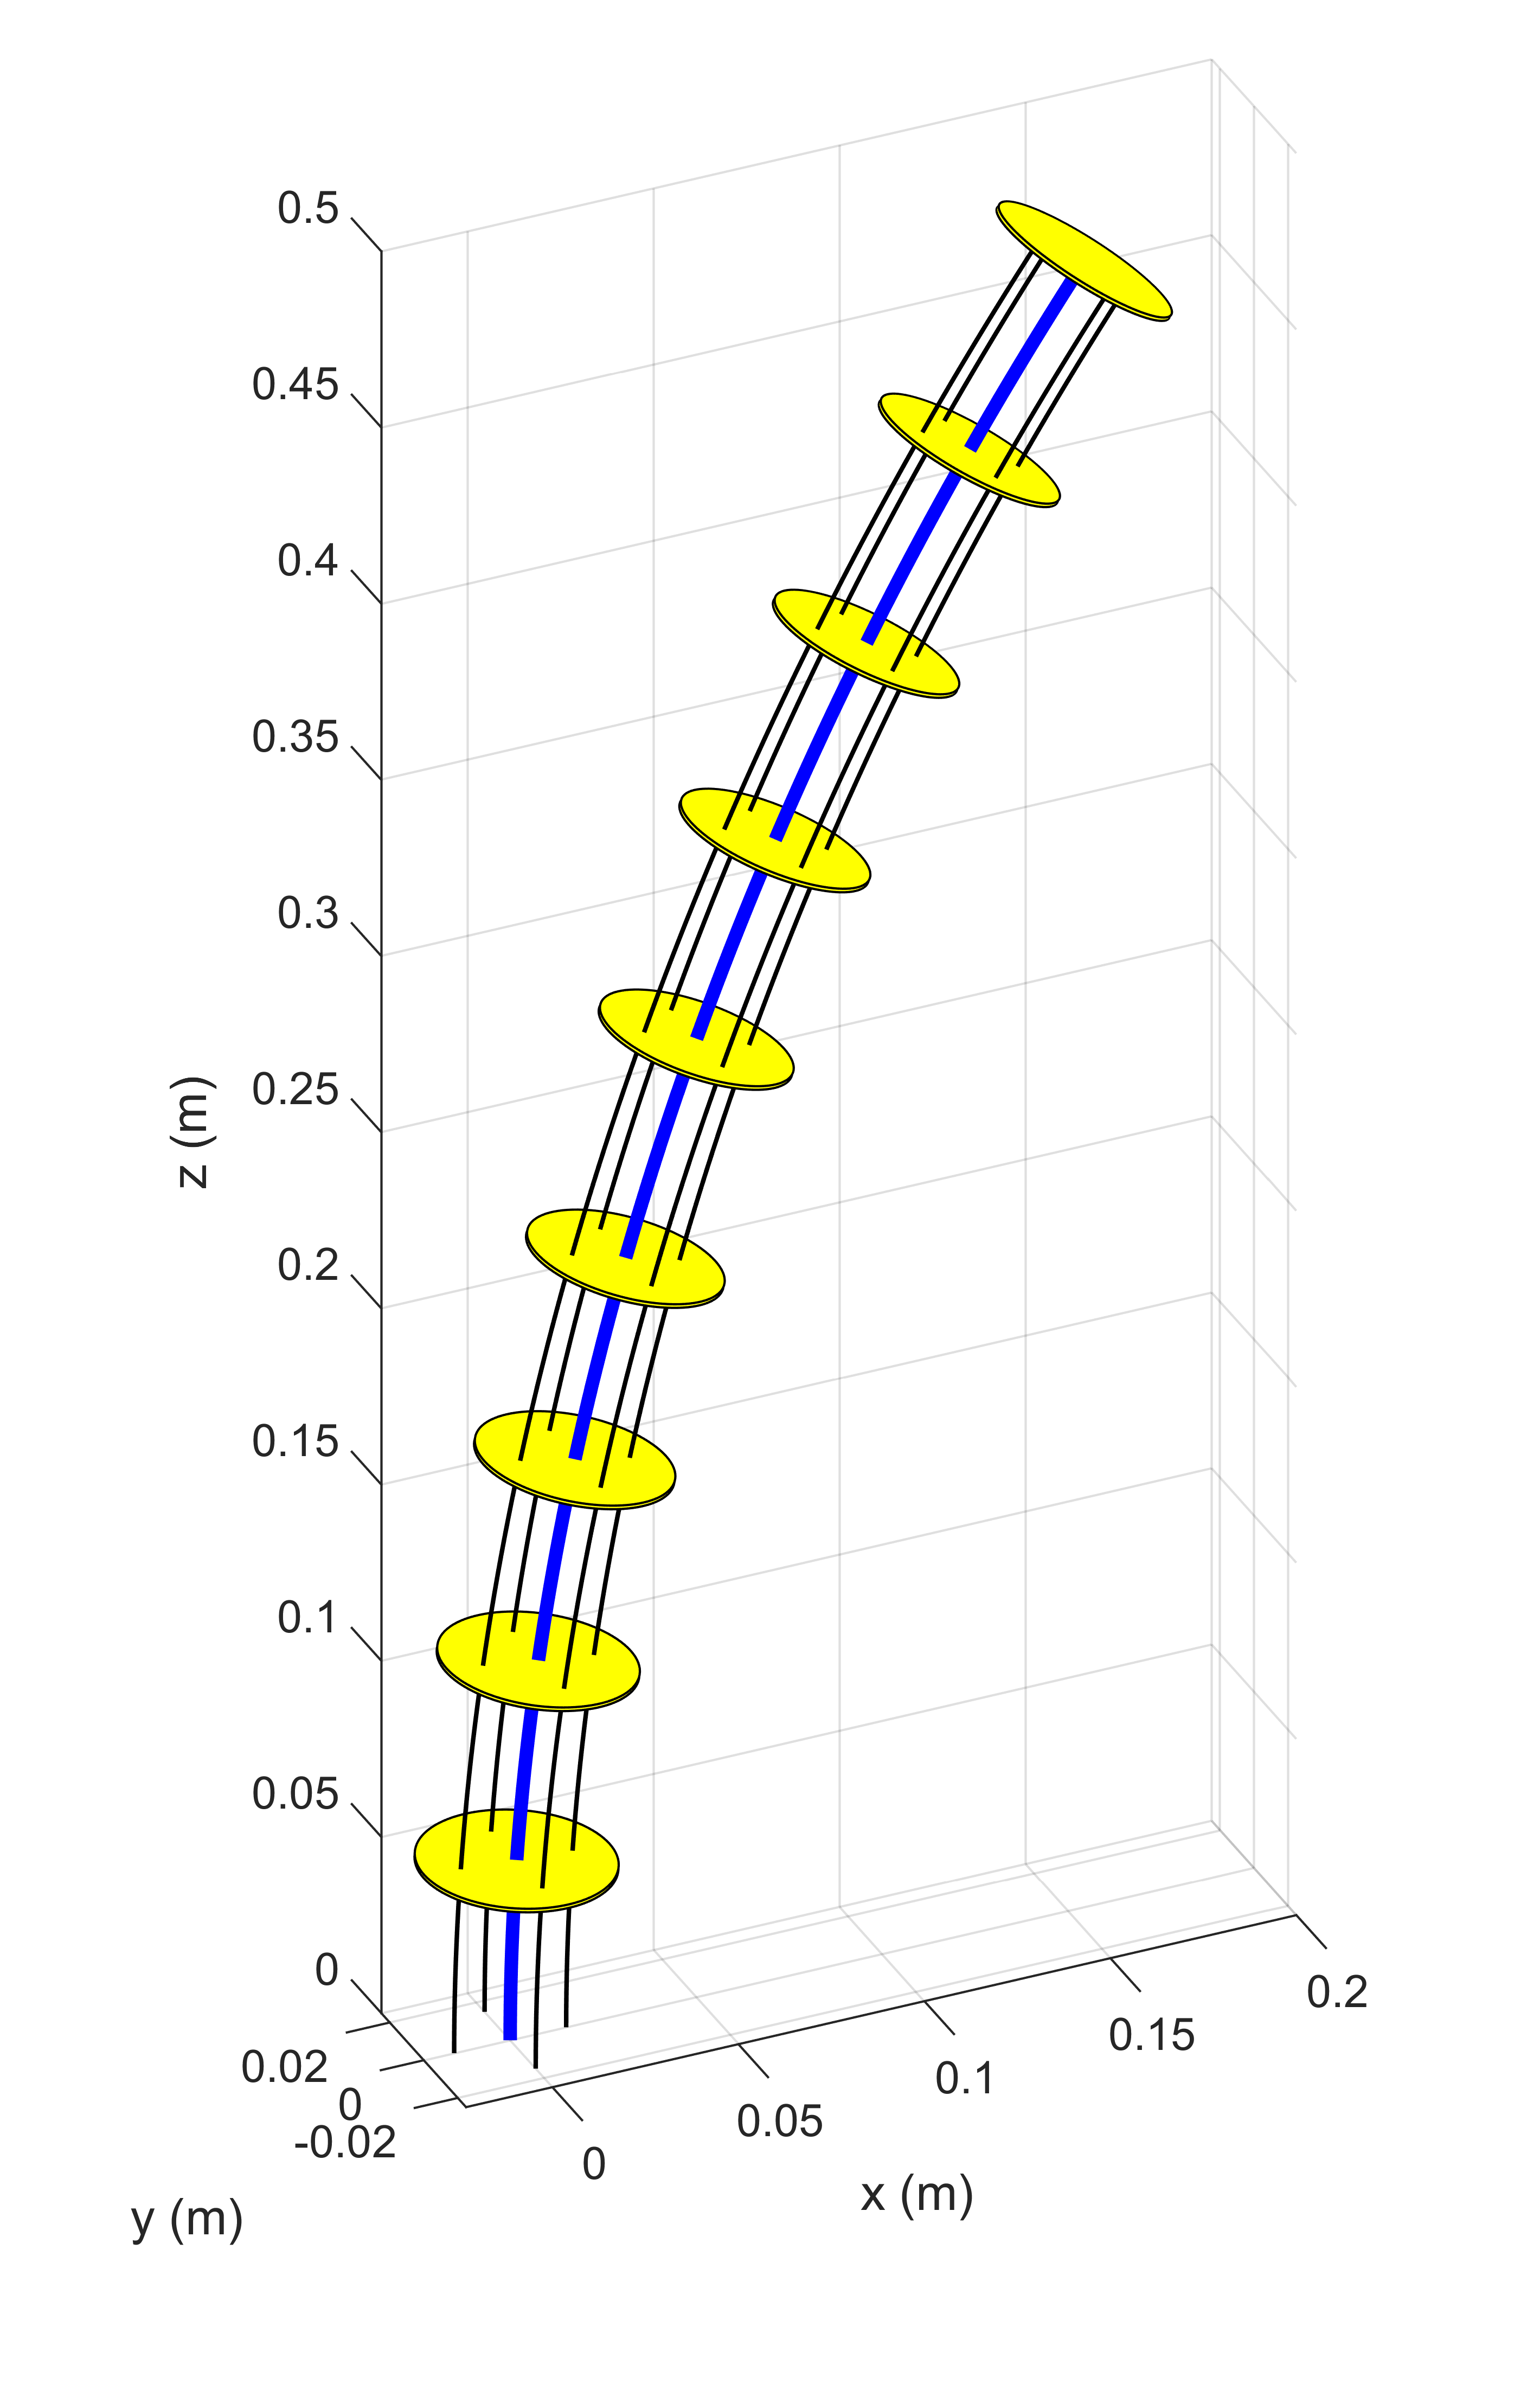
\includegraphics[width=0.5\textwidth]{fig/TendonRobotMatlab.png}
\end{figure}

\end{document}